% ---------------------------------------------------------------
% Section: Physics Analysis — ABP Model
% ---------------------------------------------------------------

\section[Physics Analysis]{Physics Analysis: Active Brownian Particle Model}

\begin{frame}{Active Brownian Particle (ABP) Model}
\begin{columns}
\begin{column}{0.50\textwidth}
\textbf{Equations of motion (2D, overdamped):}
\begin{align*}\small
    \dot{x} &= v_0 \cos\varphi + \xi_x(t) \\
    \dot{y} &= v_0 \sin\varphi + \xi_y(t) \\
    \dot{\varphi} &= \xi_\varphi(t)
\end{align*}
\small with $\langle\xi_i\xi_j\rangle = 2D_t\delta_{ij}\delta(t{-}t')$,\;
$\langle\xi_\varphi^2\rangle = 2D_r\delta(t{-}t')$.

\smallskip
\textbf{Analytical MSD:}
\begin{equation*}\small
    \langle \Delta r^2 \rangle = 4D_t\tau + \frac{2v_0^2}{D_r}\!\left[\tau - \frac{1-e^{-D_r\tau}}{D_r}\right]
\end{equation*}
\end{column}
\begin{column}{0.50\textwidth}
\textbf{Two regimes:}
\begin{itemize}\small
    \item $\tau \ll D_r^{-1}$: ballistic, MSD $\propto \tau^2$
    \item $\tau \gg D_r^{-1}$: enhanced diffusion, MSD $\propto \tau$
\end{itemize}
\smallskip
\textbf{Angular MSD (linear regime):}
\begin{equation*}\small
    \langle (\Delta\varphi)^2 \rangle = 2D_r\tau
\end{equation*}
\smallskip
\textbf{Three parameters to extract:}
\begin{itemize}\small
    \item $D_t$ — translational diffusion
    \item $v_0$ — self-propulsion speed
    \item $D_r$ — rotational diffusion
\end{itemize}
\end{column}
\end{columns}
\end{frame}

\begin{frame}{MSD Computation \& Calibration}
\begin{columns}
\begin{column}{0.55\textwidth}
\textbf{Translational MSD:}
\begin{itemize}\small
    \item Ensemble-averaged, tracks with $\geq 50$ real frames
    \item Real (non-interpolated) positions only
    \item Lag $\tau = 1\ldots100$ frames
    \item Fit via \texttt{scipy.optimize.curve\_fit}
\end{itemize}
\smallskip
\textbf{Angular MSD:}
\begin{itemize}\small
    \item \texttt{np.unwrap($\varphi$)} for phase continuity
    \item Linear fit on first 30\% of lags ($\leq$30 pts)
    \item Slope $/\, 2 = D_r$
\end{itemize}
\end{column}
\begin{column}{0.45\textwidth}
\small\begin{tabular}{|l|c|}
\hline
Pixel size & 0.078 µm/px \\
\hline
Frame rate & 30 fps \\
\hline
$\Delta t$ & $0.0\overline{3}$ s \\
\hline
\end{tabular}
\smallskip

\textbf{Pixel $\to$ physical units:}
\begin{align*}\small
    D_t &= D_t^{\rm px} \times (0.078)^2 \\
    v_0 &= v_0^{\rm px} \times 0.078 \\
    D_r &\text{ unchanged (rad}^2\text{/s)}
\end{align*}
\end{column}
\end{columns}
\end{frame}

\begin{frame}{MSD Plots — JP\_Fe\_wf\_2\_40}
\begin{figure}
    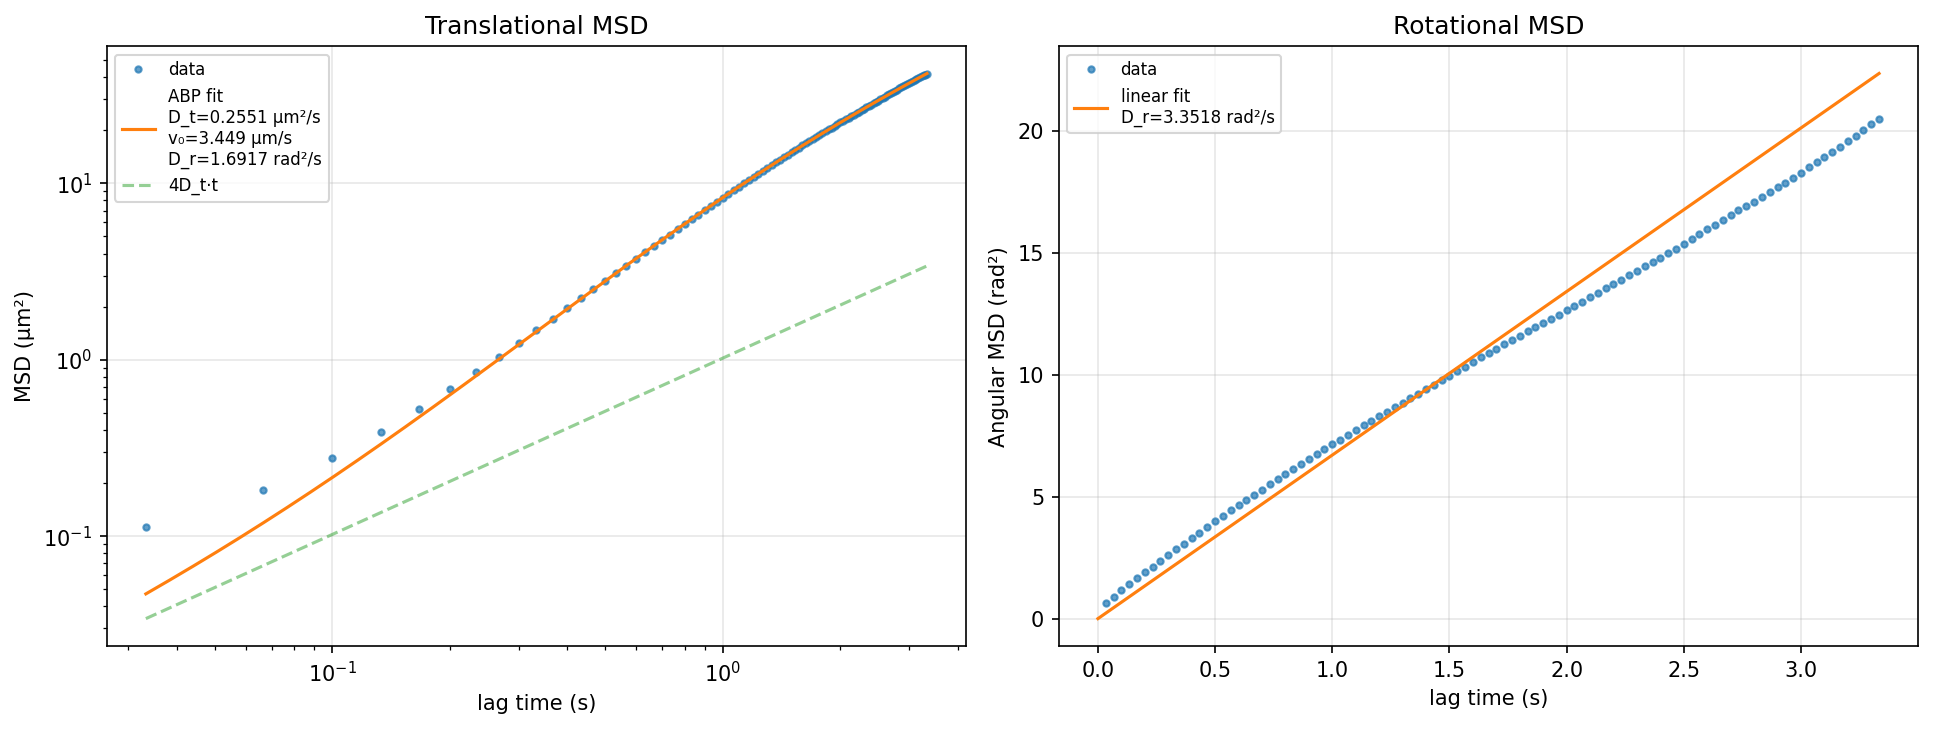
\includegraphics[width=\textwidth]{imglib/tracking/tracks_msd.png}
    \caption{\small \textit{Left}: translational MSD with ABP fit and $4D_t\tau$ reference. \textit{Right}: angular MSD with linear fit.}
\end{figure}
\end{frame}

\begin{frame}{Physics Parameters — Results}
\begin{columns}
\begin{column}{0.50\textwidth}
\small\begin{tabular}{|l|l|l|}
\hline
\textbf{Param.} & \textbf{Value} & \textbf{Method} \\
\hline
$D_t$ & 0.255 µm²/s  & ABP MSD fit \\
\hline
$v_0$ & 3.45 µm/s   & ABP MSD fit \\
\hline
$D_r$ & 1.69 rad²/s & ABP MSD fit \\
\hline
$D_r$ & 3.35 rad²/s & Angular MSD \\
\hline
\end{tabular}

\end{column}
\begin{column}{0.50\textwidth}
\textbf{Interpretation:}
\begin{itemize}\small
    \item $D_t$ consistent with Stokes-Einstein ($R\approx0.75$ µm Fe sphere)
    \item $v_0 = 3.45$ µm/s typical for magnetically driven JP (1–20 µm/s)
    \item $D_r$ factor-2 discrepancy: NCC quantisation noise inflates angular MSD slope
\end{itemize}
\end{column}
\end{columns}
\end{frame}
